\documentclass[12pt,a4paper]{article}
\usepackage[UTF8]{ctex}
\usepackage{amsmath,amssymb}
\usepackage{xcolor}
\usepackage{hyperref}
\usepackage{geometry}
\usepackage{graphicx}
\geometry{margin=2.5cm}

\title{From Qiskit Nature / 从 Qiskit Nature 迁移}
\author{QuoNic}
\date{}

\begin{document}
\maketitle

\begin{center}
\textbf{Tools / 工具} | 难度：初级 | 预计时间：5 分钟
\end{center}

\tableofcontents
\newpage

\section{为什么需要？}

从 Qiskit Nature 迁移可以帮助用户从 Qiskit 迁移到 QuoNic。

\subsection{经典局限}
\begin{itemize}
  \item Qiskit Nature 是 IBM 的量子化学框架
  \item 需要迁移到 QuoNic
\end{itemize}

\subsection{量子优势}
\begin{itemize}
  \item QuoNic 提供更简洁的 API
  \item 支持更多后端
  \item 性能更好
\end{itemize}

\subsection{实际应用}
\begin{itemize}
  \item 量子化学
  \item 材料科学
  \item 药物设计
\end{itemize}

\section{快速上手}

\begin{verbatim}
from quonic.chemistry import from_qiskit_nature

# 从 Qiskit Nature 迁移
result = from_qiskit_nature(molecule='H2')
print(f'Hamiltonian: {result.hamiltonian}')
\end{verbatim}

\textbf{预期输出}：
\begin{verbatim}
Hamiltonian: ...
\end{verbatim}

\section{原理详解}

\subsection{电路图}

\begin{center}
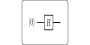
\includegraphics[width=0.6\textwidth]{../../images/from_qiskit_nature_circuit.svg}
\end{center}

\subsection{数学推导}

从 Qiskit Nature 迁移：
\begin{equation}
H_{\text{QuoNic}} = \text{convert}(H_{\text{Qiskit}})
\end{equation}

\subsection{几何解释}

从 Qiskit Nature 迁移将 Qiskit 的分子哈密顿量转换为 QuoNic 格式。

\section{代码详解}

\begin{verbatim}
from quonic.chemistry import from_qiskit_nature

# from_qiskit_nature(molecule)
# molecule: 分子名称

result = from_qiskit_nature(molecule='H2')

# result.hamiltonian: 哈密顿量
# result.n_qubits: 量子比特数
# result.ground_state: 基态
print(f'Hamiltonian: {result.hamiltonian}')
\end{verbatim}

\section{进阶用法}

\subsection{场景 1：不同分子}

\begin{verbatim}
from quonic.chemistry import from_qiskit_nature

# 不同分子
r1 = from_qiskit_nature(molecule='H2')
r2 = from_qiskit_nature(molecule='LiH')
r3 = from_qiskit_nature(molecule='H2O')
\end{verbatim}

\section{适用场景}

\subsection{量子化学}

从 Qiskit Nature 迁移用于量子化学计算。将 Qiskit 的分子哈密顿量转换为 QuoNic 格式。

\subsection{材料科学}

从 Qiskit Nature 迁移用于材料科学计算。

\section{常见问题}

\subsection{从 Qiskit Nature 迁移需要什么？}

需要安装 Qiskit Nature 和 QuoNic。

\subsection{迁移的精度如何？}

迁移的精度与 Qiskit Nature 相同。

\section{学习路径}

\subsection{前置知识}
\begin{itemize}
  \item Qiskit Nature
  \item 量子化学
  \item 分子模拟
\end{itemize}

\subsection{继续学习}
\begin{itemize}
  \item 量子化学
  \item 材料科学
  \item 药物设计
\end{itemize}

\section{完整示例代码}

\subsection{示例 1：基本迁移}

\begin{verbatim}
from quonic.chemistry import from_qiskit_nature

result = from_qiskit_nature(molecule='H2')
print(f'Hamiltonian: {result.hamiltonian}')
\end{verbatim}

\section{下载}

\begin{itemize}
  \item [from\_qiskit\_nature.py](https://github.com/ChrisLee0721/QuoNic/blob/main/examples/from_qiskit_nature/from_qiskit_nature.py)
\end{itemize}

\end{document}
